\graphicspath{{figures/design/}}
\chapter{Design}\label{ch:design}
Based on the acquired knowledge from \autoref{ch:analysis} and \autoref{ch:data_anal}, a design of occlusion detection solutions are made. This is implemented using Python3 with the Keras API working with Tensorflow.

This chapter gives an in-depth description of how the implementations are made and the theory behind them.\\

As stated in \autoref{ch:analysis} the use of \gls{cnn}s in object detection is the highest performing solution in different benchmarks. Due to this it is chosen to utilise \gls{cnn}s to perform the occlusion detection of zebrafish. In the following, a description of \gls{cnn}s in general and of the implementation for occlusion detection is presented.

\section{Convolutional Neural Networks (CNN)}
As regular neural networks, \gls{cnn}s are made up of neurons which have learnable weights and biases. Each neuron in the network receives inputs, performs an operation on the input and passes the output on, either linearly or non-linearly, dependent on the design.\\

A \gls{cnn} receives an input image and then transforms this through a series of hidden layers in the network. Each hidden layer consist of a set of neurons, and each neuron is fully connected to the neurons in the previous layer, but does not share any connections inside the layer. The last layer, the output layer, is a fully connected layer and represents the class scores. A \gls{cnn} has neurons arranged in three dimensions, namely: width, height, and depth. Already in the input an RGB image will have a depth of three due to the three colour channels \citep{Karpathy2016b}. A small example of the \gls{cnn} architecture is shown in \autoref{fig:cnn_arch}.

\begin{figure}[H]
	\centering
	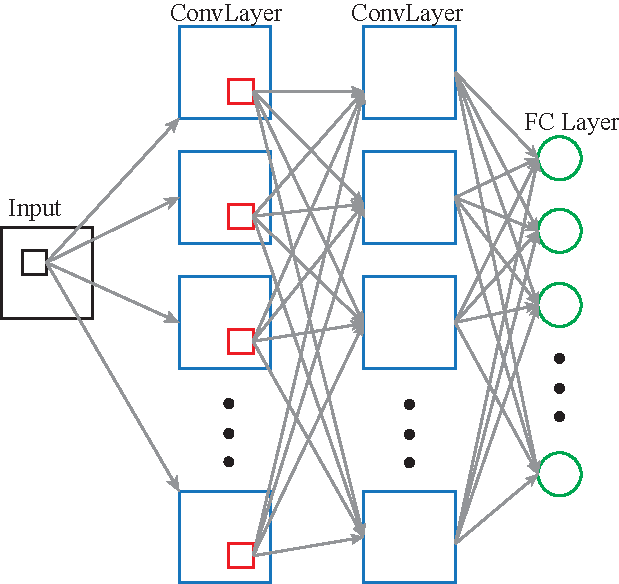
\includegraphics[width=0.6\textwidth]{cnn_arch}
	\caption{Example of a \gls{cnn} architecture}
	\label{fig:cnn_arch}
\end{figure}

\subsection{Layers}
A simple \gls{cnn} will often consist of a sequence of layers, in which each layer transforms one volume of activations to another through differentiable functions. The main layers used are; convolutional layer, pooling layer, and fully connected layer. These layers are presented in the following.

\subsubsection{Convolutional Layers}
The convolutional layer is the main layer of operations in a \gls{cnn}, hence the name of the network type.\\

A convolutional layer operates using a filter also known as a kernel to compute an output by iterating through the input image. This filter convolutes the input using the kernel weights to calculate a dot product of the input. Each filter produces a 2-dimensional activation map. If multiple filters are applied, the 2D activation maps will be stacked along the depth dimension in the output .

Besides being able to control the width and height of the kernel, most often a square, it is also possible to control the depth. Depth is a hyper parameter and corresponds to the amount of filters applied to the input. The neurons along the depth dimension may activate on different edges or colours, but are still focusing on the same region as the rest of the depth column.

When sliding a kernel over an input, a stride can be selected. With a stride of $1$ the filter moves only one pixel at a time, while with a stride of $2$ or higher the filter will move multiple pixels before performing a convolution again.

To enable a kernel to compute all pixels of an input, zero padding is necessary. The size of the zero padding is another hyper parameter, and it allows for controlling the size of the output, mostly for keeping the input size, in height and width, in the output \citep{Karpathy2016b}. A one dimensional example of the influences the different hyper parameters has is shown in \autoref{fig:hyper_ex}.

\begin{figure}[H]
	\centering
	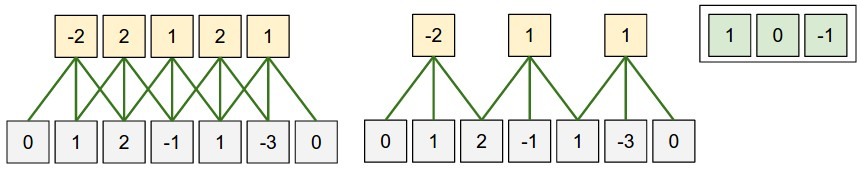
\includegraphics[width=\textwidth]{hyper_ex}
	\caption{With a kernel of [1, 0, -1] the left example shows an input in the bottom with zero padding of size 1 and stride of 1. The right convolution has changed to stride 2 \citep{Karpathy2016b}}
	\label{fig:hyper_ex}
\end{figure}

\autoref{fig:hyper_ex} shows that with a stride of one and employing zero padding, it is possible to keep the dimensions of the input in the output.

The output of a kernel can be calculated using the \autoref{eq:kernel_out}:

\begin{equation}\label{eq:kernel_out}
	(W-F+2P)/S+1
\end{equation}
Where $ W $ is the input volume size, $F$ is the kernel size, $P$ is the amount of zero padding used on the border of the input and, $S$ is the stride. Using the example in \autoref{fig:hyper_ex}, the output can be calculated: 
\begin{equation}
(5-3+2\cdot1)/1+1=5
\end{equation}

The application of stride has some limitations, as the result of \autoref{eq:kernel_out} has to be an integer \citep{Karpathy2016b}.\\

\subsubsection{Pooling Layers}
To be able to control overfitting and to reduce the amount of parameters thereby the computations in a network, pooling layers are often periodically placed in-between successive convolutional layers. A pooling layer reduces the spatial size of the input.

The size reduction is done using a filter in the same way as with a convolutional filter, but no convolutions are performed, instead, dependent on the kind of pooling, a value inside the filter is chosen to be passed on to the ooutput map. Using the most common type of pooling, Maxpooling, often with a filter size of $2\times2$ and a stride of 2, the highest pixel value within the filter is chosen as the output \citep{Karpathy2016b}. An example of this is shown in \autoref{fig:maxpool}.

\begin{figure}[H]
	\centering
	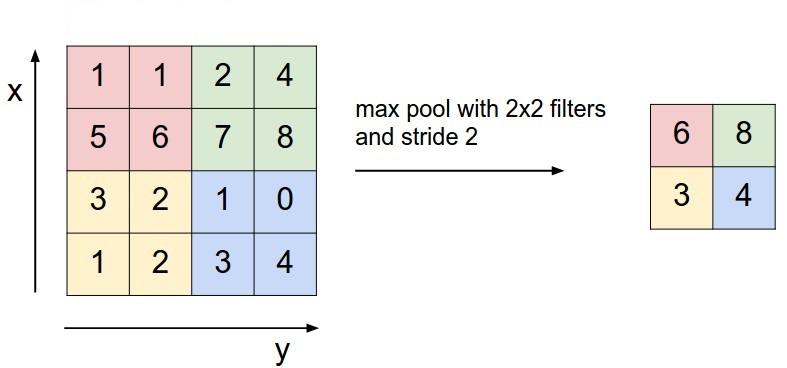
\includegraphics[width=0.8\textwidth]{maxpooling}
	\caption{Maxpooling example with a $2\times2$ kernel and stride 2 \citep{Karpathy2016b}}
	\label{fig:maxpool}
\end{figure}

\subsubsection{Classification}
To be able to use the features extracted from input image in the convolutional layers one or more \gls{fc} layers are added in the end of a \gls{cnn}. As the name suggests, all the neurons in the previous layer are connected to the \gls{fc} layer.

To classify $N$ number of classes, the last \gls{fc} layer has the same amount of neurons as the amount of classes. The output of the last \gls{fc} layer is then the probability of the input image belonging to each class, with a sum of all output neurons being $1$ \citep{Karpathy2016b}.


%\section{Faster R-CNN}
%To be able to detect objects in a frame using a \gls{cnn} the Faster R-\gls{cnn} proposed by \cite{Ren2017} is used. The chosen solution model is the third iteration of the Region based Convolutional Neural Network by \cite{Girshick2014}. As the title proposes, the network is a region proposal based network, used for object detection in an image.

%\subsection{Object Detection}
%Object detection opposed to image classification aims to locate defined objects or instances in images, and often in images containing several objects to locate at the same time, whereas an image classification solution aims to classify one object in an image and recognise the the single object without any localisation.
%
%\subsection{Region-based Convolutional Neural Network (R-CNN)} 
%The model for the R-\gls{cnn} begins with a region search and then do the classification. This model uses \textit{Selective Search} which initialises regions in the image and then merge these with a hierarchical grouping. The final grouping is then a box containing the entire image. The regions are grouped in relation to colour space and similarity \citep{Girshick2014}.
%
%The regions proposed are then fed into the \gls{cnn} which in this case extracts a $4096$ dimensional feature vector. From this feature vector a classification is done using an \gls{svm} for each class \citep{Girshick2014}. \autoref{fig:rcnn_flow} shows the steps in the R-\gls{cnn}.
%
%%\begin{figure}[H]
%%	\centering
%%	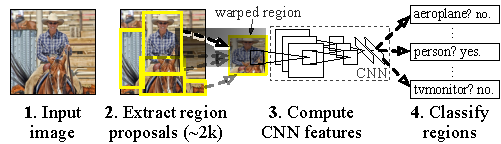
\includegraphics[width=0.8\textwidth]{rcnn_flow}
%%	\caption{Simple flow diagram of the R-\gls{cnn} by \cite{Girshick2014}}
%%	\label{fig:rcnn_flow}
%%\end{figure}
%
%The solution pre-trained on the ImageNet 2012 dataset and is fine tuned using an \gls{iou} greater than $0.5$ with the ground-truth boxes. At the time of development, \cite{Girshick2014} achieves a $62.4\%$ \gls{map} on the Pascal VOC 2012 dataset and $31.4\%$ \gls{map} on the ImageNet 2013 dataset, achieving top position on the leader boards for both datasets.
%
%\subsection{Fast Region-based Convolutional Network (Fast R-CNN)}
%The next iteration of the model by \cite{Girshick2015} is made to reduce time consumption due to the amount of models used to analyse all the regions proposed in the R-\gls{cnn}.
%
%Instead of using the selective search on the entire image, a \gls{cnn} is used to extract features from the image, and the selective search is utilised to detect \gls{roi}s from the feature maps produced by the \gls{cnn} \citep{Girshick2015}.
%
%\subsection{Faster Region-based Convolutional Network (Faster R-CNN)}
%The third iteration of R-\gls{cnn} replaces the selective search with a \textit{Region Proposal Network (\gls{rpn})}, which is a network that generates regions proposals, predict bounding boxes and detects objects.
%
%Here, once again, a \gls{cnn} is used to produce feature maps from the entire image and then uses the \gls{rpn} to propose regions and feed these to a classifier.
%
%The Faster R-\gls{cnn} outperforms the previous iterations in both accuracy and speed. Due to this, the Faster R-\gls{cnn} solution is chosen to utilise for an occlusion detection model.
\section{Image Classification}
A simple occlusion detection can be made without any localisation in order to notify a system of an occlusion present in an image. This is done using an image classification network, trained on two classes; \textit{occlusion} or \textit{no occlusion}.

The network chosen is the VGG16 network, as this is also what the \gls{rcnn} classification network is based upon. An overview of the layers in the VGG16 network is shown in \autoref{fig:vgg16}.

\begin{figure}[H]
	\centering
	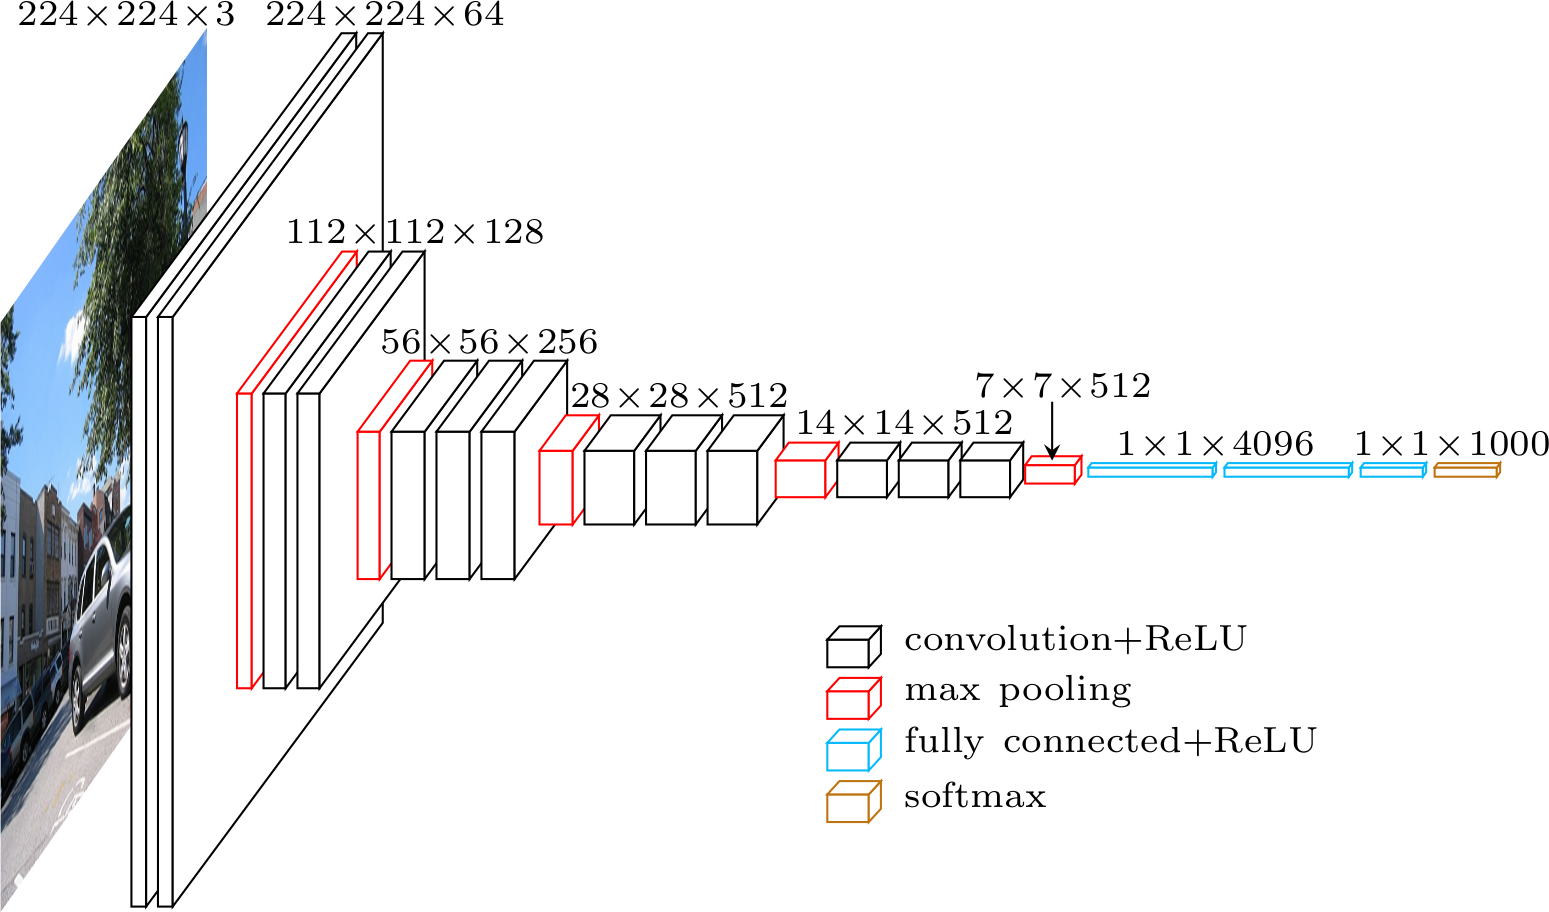
\includegraphics[width=\textwidth]{vgg}
	\caption{VGG16 structure}
	\label{fig:vgg16}
\end{figure}

The network is trained with the pre-trained weights from the ImageNet database. The network can be split into five blocks of convolutions with a max pooling layer after each block.

The images fed into the network are of size $224 \times 224$ and the last fully connected layer has a depth of $2$ due to the amount of classes. The structure of the network is shown in \autoref{tab:vgg16}. \autoref{tab:vgg16} also shows an extra dense layer has been added, and the depth of the \gls{fc} layers has been made smaller.

\begin{table}[H]
	\centering
	\caption{Detailed description of VGG16 design. The input is $224 \times 224 \times3$ images}
	\label{tab:vgg16}
 	\begin{tabular}{lrrrr}
		\textbf{Layer Type}     & \textbf{Feature Map Size} & \textbf{Kernel/Pool Size} & \textbf{Activation}  \\ \hline
		\textbf{Block 1}        &                           &                           &                                     \\
		\rowcolor{lightGrey}  
		Conv2D                  & $64$                      & $3\times3$                & ReLU                                \\
		Conv2D                  & $64$                      & $3\times3$                & ReLU                                \\
		\rowcolor{lightGrey} 
		MaxPooling2D            &                           & $2\times2$                &                                     \\
		\textbf{Block 2}        &                           &                           &                                     \\
		\rowcolor{lightGrey}  
		Conv2D                  & $128$                     & $3\times3$                & ReLU                                \\
		Conv2D                  & $128$                     & $3\times3$                & ReLU                                \\
		\rowcolor{lightGrey}  
		MaxPooling2D            &                       &    $2\times2$             & ReLU                                \\
		\textbf{Block 3}        &                           &                           &                                    \\
		\rowcolor{lightGrey}  
		Conv2D                  & $256$                     & $3\times3$                & ReLU                                \\
		Conv2D                  & $256$                     & $3\times3$                & ReLU                                \\
		\rowcolor[HTML]{EFEFEF} 
		Conv2D                  & $256$                     & $3\times3$                & ReLU                                \\
		MaxPooling2D            &               &          $2\times2$                  &                                     \\
		\textbf{Block 4}        &                           &                           &                                     \\
		\rowcolor{lightGrey}  
		Conv2D                  & $512$                     & $3\times3$                & ReLU                                \\
		Conv2D                  & $512$                     & $3\times3$                & ReLU                                \\
		\rowcolor{lightGrey}  
		Conv2D                  & $512$                     & $3\times3$                & ReLU                                \\
		MaxPooling2D            &             &          $2\times2$                  &                                     \\
		\textbf{Block 5}        &                           &                           &                                    \\
		\rowcolor{lightGrey}  
		Conv2D                  & $512$                     & $3\times3$                & ReLU                                \\
		Conv2D                  & $512$                     & $3\times3$                & ReLU                                \\
		\rowcolor{lightGrey}  
		Conv2D                  & $512$                     & $3\times3$                & ReLU                                \\
		MaxPooling2D            &               &        $2\times2$        & ReLU                                \\
		\textbf{Classification} &                           &                           &                                     \\
		\rowcolor{lightGrey}  
		Flatten                 &                           &                           &                                     \\
		Dense                   & $1024$                    &                           & ReLU                                \\
		\rowcolor{lightGrey}  
		Dense               	& $1024$                    &                           & ReLU                 	           \\
		Dense                   & $512$                    	&                           & ReLU                                \\
		\rowcolor{lightGrey} 
		Dense                   & Amount of Classes         &                           & Softmax                            
	\end{tabular}
\end{table}

\section{Faster \gls{rcnn} Object Detection}
To be able to localise the occlusions in the image and mark them with bounding boxes, an object detection solution is necessary. For this the Faster \gls{rcnn} presented in \autoref{ch:analysis} is implemented. In the following the different objects in the pipeline are described in more detail. An example overview of the pipeline is shown in \autoref{fig:faster_rcnn}.

\begin{figure}[H]
	\centering
	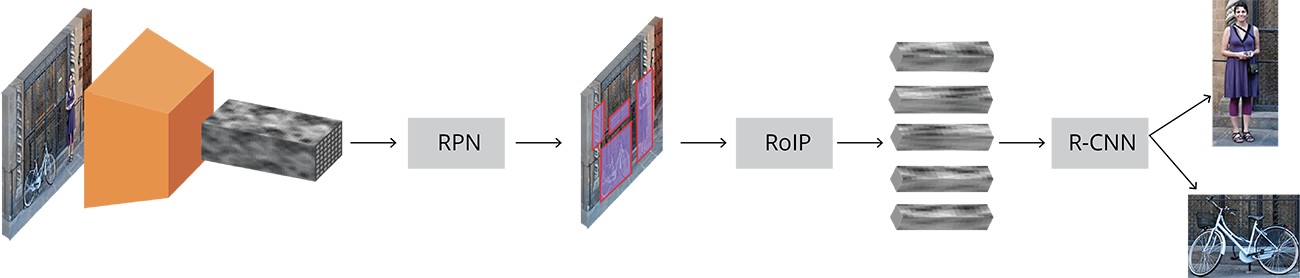
\includegraphics[width=0.9\textwidth]{fasterrcnn-architecture}
	\caption{Overview of the Faster \gls{rcnn} pipeline and its steps \citep{Rey2018}}
	\label{fig:faster_rcnn}
\end{figure}


\subsection{Region Proposal Network}
As mentioned in \autoref{sec:obj_det} \nameref{sec:obj_det}, the Faster \gls{rcnn} utilises a network called \textit{\gls{rpn}} to produce region proposals. The \gls{rpn} shares some convolutional layers with the \gls{cnn}. By sliding a small network over the feature map produced by the last shared convolutional layer \citep{Ren2017}.

As the objective of the object detection is to find bounding boxes in the image, anchors are used. Anchors are fixed bounding boxes of different sizes and ratios and are placed throughout the image. They are used for reference when predicting object locations. An anchor is created for each point in the produced feature map, but the final anchors still reference the input image of the network. The \gls{rpn} outputs a set of good proposals based on the anchors, by having two outputs for each. The first output is an object probability score, the second is bounding box regression for adjusting the anchors to fit potential objects. An example of how anchors are placed in an input image is shown in \autoref{fig:anchors}.

\begin{figure}[H]
	\centering
	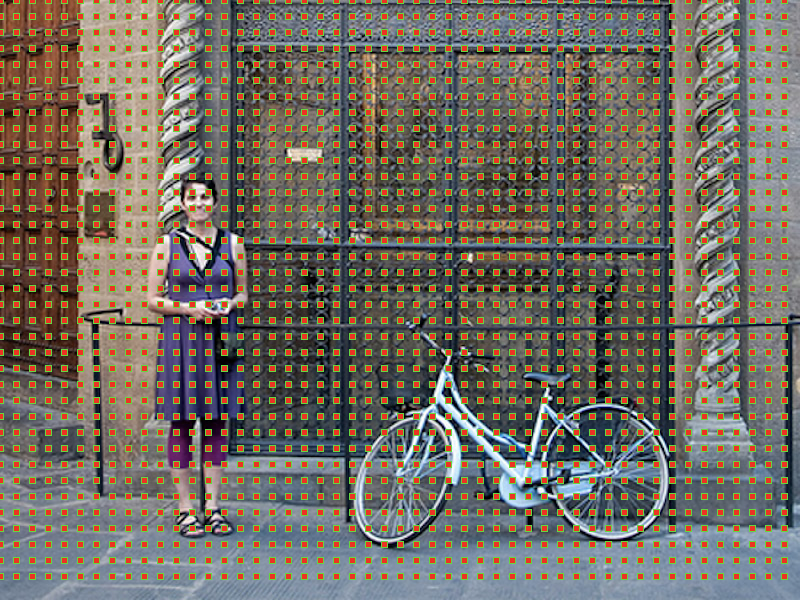
\includegraphics[width=0.6\textwidth]{anchors-centers}
	\caption{Example of anchor centres placed in an input image \citep{Rey2018}}
	\label{fig:anchors}
\end{figure}

For training the \gls{rpn}, the anchors are split into two different categories; the first are those which overlap a ground-truth object with an \gls{iou} of more than $0.7$ which are considered foreground or an object. The second category are those that do not overlap a ground-truth object or have less than $0.3$ \gls{iou}, and are considered background. 
A batch of the anchors is sampled, maintaining a balance between foreground and background anchors. This batch is used to calculate the classification loss using binary cross entropy, and the foreground anchors, only, of the batch to calculate regression loss \citep{Ren2017}.\\

In post processing, \gls{nms} is applied to solve duplicate proposals of one object by discarding the proposals with an \gls{iou} above a set threshold with another proposal with a higher score. A too high \gls{iou} threshold may lead to too many proposals, and too low can lead to missing proposals \citep{Ren2017}.

\subsection{Region of Interest Pooling}
With the object proposals from the \gls{rpn}, the next step is to classify the bounding boxes. But before the classification is done, \gls{roi} pooling is performed. This is done by extracting the fixed size feature maps for each proposal from the already existing convolutional feature map shared \citep{Ren2017}.

\subsection{Classification}
In the classification step of the network the \gls{rcnn} network is employed. With a \gls{fc} layer as output the \gls{rcnn} has two goals; classifying the proposals into classes and to fit the bounding boxes. It flattens the feature map of each proposal and then uses two \gls{fc} layers of size $4096$ with \gls{relu} activation. Then, using two different \gls{fc} layers for each of the objects, one for classification and one for bounding box regression prediction \citep{Ren2017}. An example of the flow of a classification by the \gls{rcnn} is also shown in \autoref{fig:rcnn_ex}. Here a bicycle is classified and the bounding box is adjusted to fit the object.

\begin{figure}[H]
	\centering
	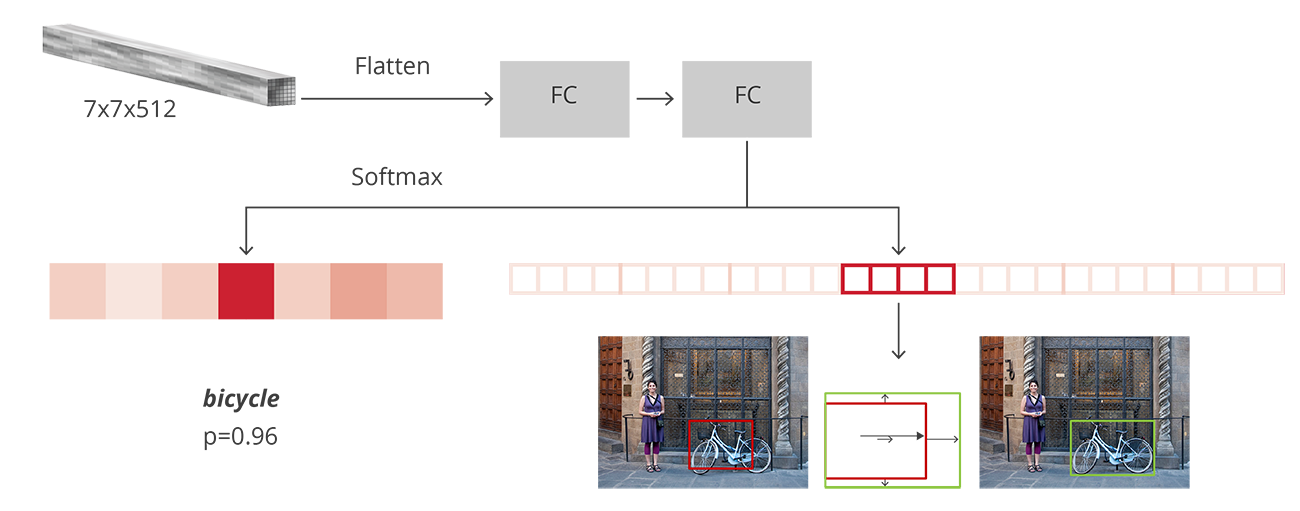
\includegraphics[width=\textwidth]{rcnn-architecture}
	\caption{Example of classification flow in the \gls{rcnn} classifying a bicycle and regressing a bounding box \citep{Rey2018}}
	\label{fig:rcnn_ex}
\end{figure}
